\documentclass[12pt,a4paper,oneside]{ctexart}
\usepackage{amsmath, amsthm, amssymb, graphicx, float, listings, xcolor}
%51汇编设置
\lstdefinelanguage{MCS51}{
  keywords={MOV, ADD, SUBB, JMP, LCALL, RET, ORL, ANL, XRL, CJNE, DJNZ, INC, DEC, SETB, CLR}, % MCS-51 指令
  keywordstyle=\color{blue}\bfseries,
  comment=[l]{;}, % MCS-51 注释
  commentstyle=\color{gray}\ttfamily,
  stringstyle=\color{red}\ttfamily,
  basicstyle=\ttfamily\footnotesize,
  morecomment=[s]{/*}{*/},
  morestring=[b]',
  morestring=[b]"
}


%导言区
\title{课程《微机原理》笔记}
\author{NH5}
\date{更新于2025.3.15}

\begin{document}
\maketitle
\textbf{本课程基于MCS51芯片}

\section{微机概述}
\subsection{微处理器}
计算机与微控制器在控制方面的差别(简答题):

1.PC机在数据处理方面的能力大大超过了微控制器,这是微控制器无法与PC机比拟的.
因此微控制器就不适合于离线应用场合:控制CAD、建模、仿真、辅助设计、大容量数值处理

2.微控制器主要是针对以对象控制为主,数值处理为辅的小型化、嵌入型控制系统中.
正因如此,微控制器中的数据存储器RAM往往很小

\subsection{冯$\cdot$诺伊曼结构与哈佛结构}
存储器结构一般有两种:普林斯顿(Princeton,又称冯$\cdot$诺伊曼结构)结构和哈佛(Harvard)结构.通用微型计
算机一般采用普林斯顿(Princeton)结构,将程序和数据合用一个存储器空间,在使用时才
分开;单片机一般采用哈佛(Harvard)结构,将程序和数据分别用不同的存储器存放,各有
自己的存储空间,分别采用不同的寻址方式.存放程序的存储器称为程序存储器,存放数
据的存储器称为数据存储器.
\begin{figure}[H]
    \centering
    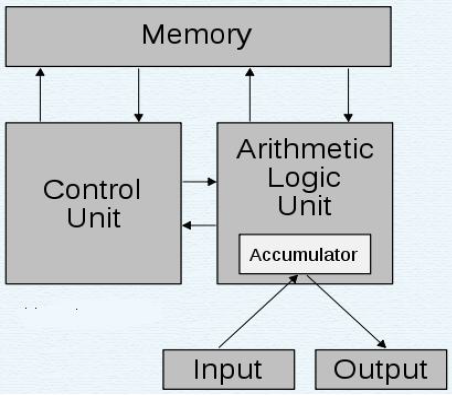
\includegraphics[width=8cm]{photos/冯诺依曼结构.png}
    \caption{冯诺依曼结构}
\end{figure}
\begin{figure}[H]
    \centering
    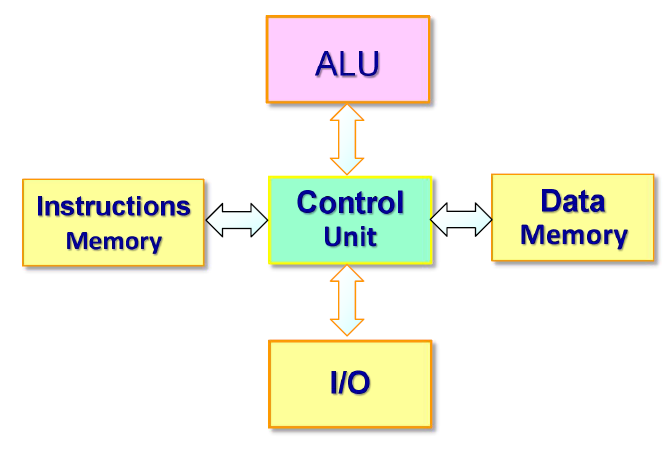
\includegraphics[width=8cm]{photos/哈佛结构.png}
    \caption{哈佛结构}
\end{figure}

\subsection{指令集}
计算机可以根据指令集分为:
精简指令计算机RISC(Reduced InstructionSet Computer)和复杂指令计算机CISC (Complex Instruction Set Computer).
RISC和CISC是目前设计制造微处理器的两种典型技术.

CISC属于早期传统计算机结构的指令体系,认为指令系统越丰富、越复杂,功能越强大,
但统计结果表明:使用的80\% 的指令,只占指令系统的20\%,
同时最频繁的指令是数据传输、算术运算等简单指令.(MCS-51属于这一类)

RISC结构优先选取使用频最高的简单指令,避免复杂指令;
将指令长度固定,指令格式和寻址方式种类减少;
以控制逻辑为主,不用或少用微码控制等.

\section{MCS51内部结构}
MCS51由下列模块构成:

1.中央处理单元CPU(8位):计算+控制的核心单元

2.程序存储器ROM(=硬盘):用于永久性存储应用程序

3.数据存储器RAM(=内存):用于程序运行中存储工作变量和数据

4.并行输入/输出(I/O口):与外界的接口(系统总线、扩展外存、外设接口)

5.串行输入/输出口(UART)(二线):与外界的串行通信

6.定时/计数器:它与CPU之间各自独立工作,当它计数满时向CPU中断

7.时钟电路(fosc):分为内部振荡器、外接振荡电路

8.中断系统:中断源、两级优先,可编程进行控制

9.内部总线:连接上述部件的通道
\begin{figure}[H]
    \centering
    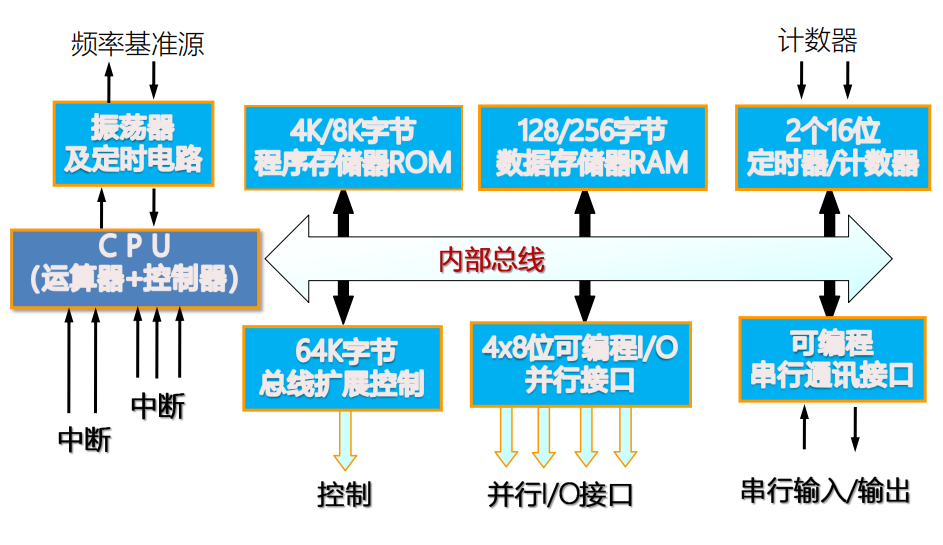
\includegraphics[width=8cm]{photos/MCS51结构.png}
\end{figure}

8051微控制器功能模块与特点:

4个8位I/O口:P0、P1、P2、P3,具有第二功能

中断系统:具有5个中断源,2个中断优先权

定时器/计数器:有2个16位的定时器/计数器,具有4种工作方式

串行接口:1个全双工的串行口,用于微控制器与具有串行接口的外设进行异步串行通信,也可以扩展I/O接口

布尔处理器:具有较强的位寻址、位处理能力

时钟电路:产生微控制器工作所需要的时钟脉冲(需要外接晶体振荡器和微调电容)

指令系统:有5大功能,111条指令.为复杂指令系统(CISC)

\subsection{CPU}
CPU内部结构如下图:
\begin{figure}[H]
    \centering
    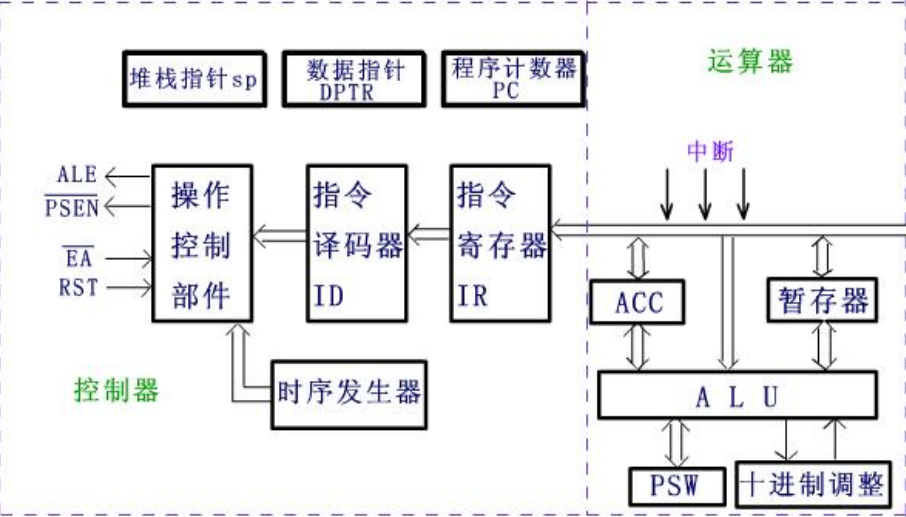
\includegraphics[width=8cm]{photos/CPU结构图.png}
\end{figure}
\subsubsection{控制器}
控制器由操作控制部件、时序发生器、指令寄存器IR、指令译码器ID、指令计数器PC等组成

控制器是CPU的大脑中枢,是识别指令,控制计算机各部分工作的部件,
包括控制取指令、译码和执行三个步骤的全部控制

指令计数器PC:

它是16位的按机器周期自动增1计数器

总指向下一条指令所在首地址(当前PC值)

一切分支/跳转/调用/中断/复位等操作的本质就是:改变PC值

用户不可读写

PC值的范围为0000H$\to$FFFFH,即可寻址范围为64K

存在PC值跳转,会用到栈来存放PC值

\subsubsection{运算器}
运算器的任务是数据的处理和加工.
由算术逻辑单元ALU、累加器Acc、暂存寄存器、程序状态寄存器PSW、布尔处理器、BCD码运算调整电路等通过内部总线连接而成

ALU:

完成算术运算及与、或 、非、异或等逻辑操作,
并通过对运算结果的判断,影响程序状态寄存器PSW相关位的状态

位处理器(布尔处理器):

能直接对位(bit)进行操作,操作空间是位寻址空间.
位处理器中功能最强、使用最频繁的位是C,也称其为位累加器

暂存寄存器:

用于运算数据的暂时存放,该寄存器不能访问

累加器ACC:

存放操作数与运算结果.
51中基本上所有与计算有关的操作都要涉及到A(ACC)

以下是一个累加器的操作示例:
\begin{lstlisting}[language=MCS51]
    MOV A, 40H ;把地址40H中的数字放入A中
    ADD A, 41H ;41H中的数字与A中数字相加,结果放入A
\end{lstlisting}

程序状态字:PSW用于寄存程序运行的状态信息
\begin{figure}[H]
    \centering
    
\includegraphics[width=8cm]{photos/PSW.png}
\end{figure}

C(PSW.7):进位或借位标志位.
执行算术运算和逻辑运算指令时,用于记录最高位向前面的进位或借位.
8位加法运算时,若运算结果的最高位D7位有进位,则C置1,否则C清0.
8位减法运算时,若被减数比减数小,不够减,需借位,则C置1,否则C清0.
另外,在51单片机中,该位也可作位运算器,完成各种位处理.

AC(PSW.6):辅助进位或借位标志位.
用于记录在进行加法和减法运算时,低4位向高4位是否有进位或借位.
当有进位或借位时,AC置1,否则AC清0

F0(PSW.5),F1(PSW.1):可由用户定义的标志位

RS1、RSO(PSW.4、PSW.3):寄存器组选择位,用软件置1或清0
\begin{table}[H]
    \centering
    \begin{tabular}{|c|c|c|}
    \hline
    RS1 & RS0 & 工作寄存器组      \\ \hline
    0   & 0   & 0组(00H-07H) \\ \hline
    0   & 1   & 1组(08H-0FH) \\ \hline
    1   & 0   & 2组(10H-17H) \\ \hline
    1   & 1   & 3组(18H-1FH) \\ \hline
    \end{tabular}
    \end{table}
OV(PSW.2):溢出标志位.
在加法或减法运算时,如运算的结果超出8位二进制数的范围,则OV置1,标志溢出,否则OV清0.
\end{document}